\chapter{Concetti fondamentali}
\section{Introduzione alla programmazione parallela}
Il software senza la parallelizzazione viene eseguito su una singola unità centrale di elaborazione (CPU). Il problema viene suddiviso in una serie discreta di istruzioni che vengono eseguite una dopo l'altra e una per volta come in figura \ref{fig:serial-computation}.

\begin{figure}[th]
	\centering
	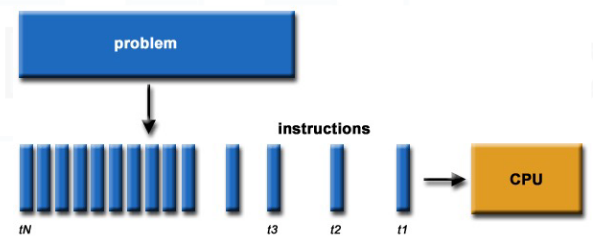
\includegraphics[width=0.8\linewidth]{img/serial-computation}
	\caption{computazione seriale.}
	\label{fig:serial-computation}
\end{figure}

Il \textbf{calcolo parallelo} consiste nell'uso simultaneo di più risorse di calcolo per risolvere un problema computazionale impiegando più CPU per eseguire le operazioni. Un problema viene suddiviso in parti più discrete, ognuna delle quali può essere risolta in modo \textbf{indipendente} e \textbf{contemporaneo}. Successivamente ogni parte è ulteriormente suddivisa in una serie di istruzioni che vengono eseguite simultaneamente su diverse CPU. Questo approccio consente di accelerare notevolmente il processo di calcolo rispetto al calcolo seriale.
\subsubsection*{Motivazioni}
\begin{enumerate}
	\item risparmiare tempo e denaro;
	\item risolvere problemi più grandi;
	\item fornire concorrenza;
	\item utilizzo di risorse non locali.
\end{enumerate}
\subsection*{Un ripasso dell'architettura di Von Neumann}

\begin{wrapfigure}{r}{0.35\linewidth}
	\centering
	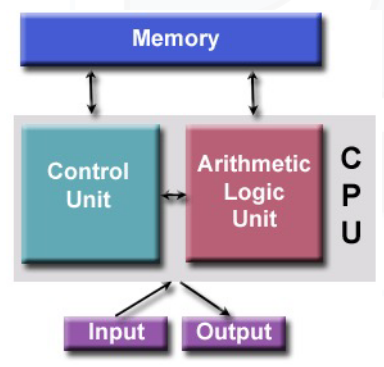
\includegraphics[width=.7\linewidth]{img/von-neumann}
	\caption{architettura di Von Neumann.}
	\label{fig:von-neumann}
\end{wrapfigure} 
Comprende la \textbf{memoria}, l'\textbf{unità di controllo}, l'\textbf{unità aritmetico logica} e le \textbf{periferiche di input/output}. La lettura e la scrittura sulla \textbf{RAM} -- \textbf{\textit{random access memory}} viene utilizzato per memorizzare sia istruzioni che dati del programma. L'\textbf{unità di controllo} recupera le istruzioni e i dati dalla memoria, decodifica le istruzioni e coordina sequenzialmente le operazioni per portare a termine il task\footnote{Generalmente con task ci si riferisce ad un compito.} programmato. L'\textbf{unità aritmetico logica} svolge le operazioni aritmetiche di base. L'\textbf{I/O} è l'interfaccia con cui avviene l'interazione uomo-macchina.

\subsection{Tassonomia classica di Flynn}
La tassonomia classica di Flynn distingue le architetture dei computer multiprocessore in base a come possono essere classificate lungo le due dimensioni indipendenti di \textbf{istruzioni} e \textbf{dati}.
\begin{figure}[th]
	\centering
	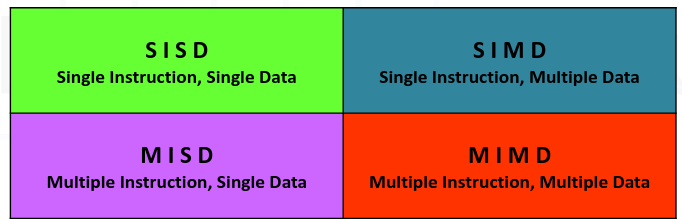
\includegraphics[width=0.7\linewidth]{img/flynn}
	\caption{matrice di flynn.}
	\label{fig:flynn}
\end{figure}

\subsubsection*{Legenda figura \ref{fig:sisd}}
\begin{enumerate}
	\item IS -- \textit{Instruction stream}. Le istruzioni di un programma da eseguire;
	\item DS -- \textit{Data Stream}. Operandi e risultati su cui il programma sta lavorando;
	\item PU -- \textit{Processing Unit}. Unità funzionale composta da ALU e registri. Esegue le istruzioni;
	\item MM -- \textit{Main Memory}. La memoria in cui vengono allocati dati e istruzioni.
\end{enumerate}
\clearpage
\subsection*{SISD -- Single Istruction Single Data}
\begin{figure}[th]
	\centering
	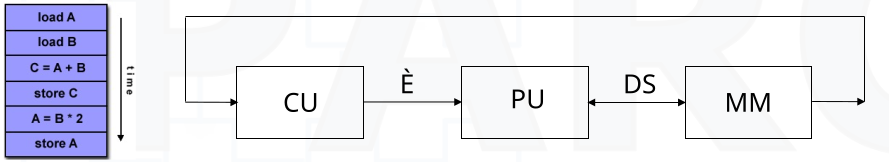
\includegraphics[width=0.7\linewidth]{img/sisd}
	\caption{sisd.}
	\label{fig:sisd}
\end{figure}\noindent
CU esegue le istruzioni dalla MM, mentre PU esegue le istruzioni interagendo con la MM per modificare i dati. È un'architettura standard di Von Neumann, in cui ciascun programma esegue e si affida ad un flusso di dati singolo. SISD è un'esecuzione seriale. Single istruction: un solo flusso di istruzioni viene elaborato dalla CPU durante un ciclo di clock. Single data: un solo flusso di dati viene utilizzato come input durante ciascun ciclo di clock. SISD fa si che l'esecuzione sia \textbf{deterministica}. SISD è presente sulle vecchie generazioni di mainframe computer, minicomputer e workstation.

\subsection*{SIMD -- Single Istruction  Multiple Data}
\begin{figure}[th]
	\begin{subfigure}{0.45\linewidth}
		\centering
		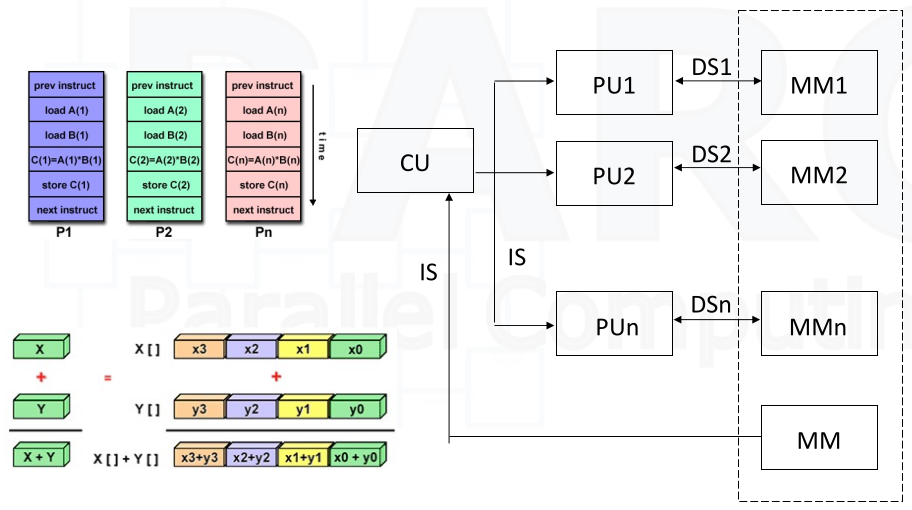
\includegraphics[width=\linewidth]{img/simd}
		\caption{simd.}
		\label{fig:simd}
	\end{subfigure}
	\hfill
	\begin{subfigure}{0.45\linewidth}
		\centering
		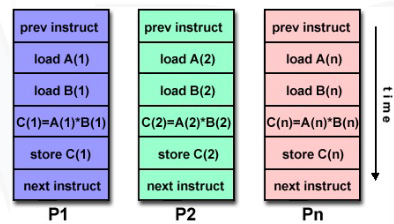
\includegraphics[width=\linewidth]{img/simd-processori}
		\caption{diversi processori eseguono la stessa istruzione su dati differenti.}
		\label{fig:simd-processori}
	\end{subfigure}
\end{figure}
SIMD è un tipo di parallel computer dove \textit{single istruction} significa che tutte le unità di elaborazione (PU) eseguono la stessa istruzione a ogni dato ciclo di clock. \textit{Multiple data} vuol dire che ogni unità di elaborazione (PU) può operare su un diverso elemento di dati. SIMD è più adatto per problemi specializzati
caratterizzati da un alto grado di
regolarità, come l'elaborazione di grafica/immagini. SIMD permette un esecuzione \textbf{deterministica} e \textbf{sincrona} (lockstep\footnote{Termine che ha origine militare, usato per riferirsi al passo sincronizzato dei soldati. In SIMD si riferisce all'esecuzione sincrona -- la CU non istruisce le PU se prima non è terminata l'elaborazione dell'istruzione precedente.}). La maggior parte dei computer moderni, in particolare quelli con unità di elaborazione grafica (GPU), impiegano istruzioni SIMD e unità di esecuzione.
\subsection*{MISD -- Multiple Instruction Single Data}

\begin{figure}[th]
	
	\begin{subfigure}{0.45\linewidth}
		\centering
		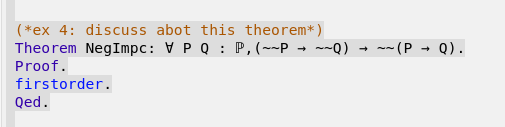
\includegraphics[width=\linewidth]{img/misd}
		\caption{misd.}
		\label{fig:misd}
	\end{subfigure}
	\hfill
	\begin{subfigure}{0.45\linewidth}
			\centering
		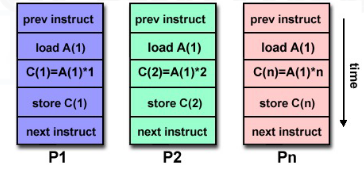
\includegraphics[width=0.7\linewidth]{img/misd-processori}
		\caption{le istruzioni sono diverse da processore a processore, ma il dato su cui operano è lo stesso.}
		\label{fig:misd-processori}		
	\end{subfigure}
\end{figure}
In MISD un singolo flusso di dati viene immesso in più unità di elaborazione. Ogni unità di elaborazione opera sui dati in modo indipendente tramite flussi di istruzioni indipendenti. Sono esistiti pochi esempi concreti di questa classe di computer paralleli. Uno è il computer sperimentale Carnegie-Mellon C.mmp (1971).

Alcuni possibili utilizzi potrebbero essere:
\begin{itemize}
	\item filtri di frequenza multipli che operano su un singolo flusso di segnale;
	\item algoritmi crittografici multipli che tentano di decifrare un singolo
	messaggio codificato.
\end{itemize}

\subsection*{MIMD -- Multiple Instruction Multiple Data}
\begin{figure}[th]
	\begin{subfigure}{0.45\linewidth}
		\centering
		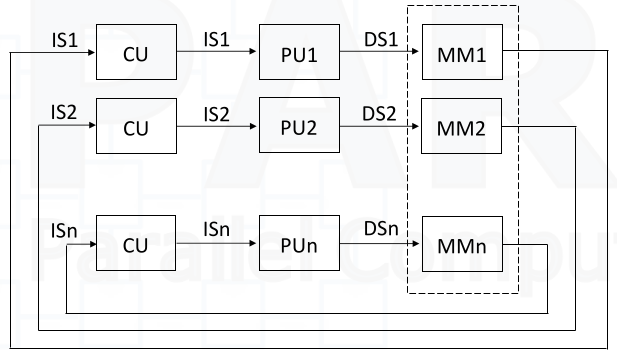
\includegraphics[width=\linewidth]{img/mimd}
		\caption{mimd.}
		\label{fig:mimd}
	\end{subfigure}
	\hfill
	\begin{subfigure}{0.45\linewidth}
		\centering
		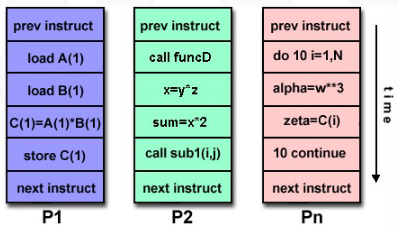
\includegraphics[width=\linewidth]{img/mimd-processori}
		\caption{istruzioni diverse vengono eseguite sui diversi processori che operano su dati differenti.}
		\label{fig:mimd-processori}
	\end{subfigure}
\end{figure}

Attualmente, il tipo più comune di computer parallelo. La maggior parte dei computer moderni rientra in questa categoria. \textit{Multiple Instruction} significa che ogni processore può eseguire un diverso flusso di istruzioni. \textit{Multiple Data} significa che ciascun processore può lavorare su un diverso flusso di dati. L'esecuzione può essere sincrona o asincrona, deterministica o non deterministica. MIMD viene utilizzata sulla maggior parte dei supercomputer attuali, cluster di computer paralleli in rete e \textit{"grid"}, computer SMP multiprocessore e PC multicore. Nota: molte architetture MIMD includono anche sottocomponenti di esecuzione SIMD.

\subsection{Terminologia delle architetture parallele}
\begin{itemize}
	\item \textbf{task}: una sezione logicamente discreta di
	lavoro computazionale. Un task è in genere un
	programma o un insieme di istruzioni simili a un programma che
	viene eseguito da un processore;
	\item \textbf{task parallelo}: un'attività che può essere eseguita da più processori in modo sicuro (produce risultati corretti);
	\item \textbf{esecuzione seriale}: esecuzione di un programma
	in sequenza, un'istruzione alla volta. Nel senso più semplice, questo è ciò che accade su una
	macchina con un solo processore. Tuttavia, praticamente tutte
	le attività parallele avranno sezioni di un programma parallelo che devono essere eseguite in serie;
	\item \textbf{esecuzione parallela}: esecuzione di un programma da parte di
	più di un task, con ogni task in grado
	di eseguire la stessa istruzione o un'istruzione diversa nello
	stesso momento;
	\item \textbf{pipelining}: suddividere un'attività in passaggi eseguiti
	da diverse unità di elaborazione, che prendono i vari flussi di input, proprio come avviene in una catena di montaggio; è un tipo di elaborazione parallela;
	\begin{figure}[th]
		\centering
		\begin{tikzpicture}
			\node[draw](A){$P_1$};
			\node[draw,right=of A](B){$P_2$};
			\node[right=of B](D){\dots};
			\node[draw, right=of D](C){$P_N$};
			\foreach \a/\b in {A/B,B/D,D/C}{
				\draw[-stealth,label distance=0.3pt, label=I/O] (\a)--(\b) node[pos=0.5,above]{I/O};
			}
		\end{tikzpicture}
		\label{fig:pipeline}
		\caption{pipeline.}
	\end{figure}
	\item \textbf{memoria condivisa}: da un punto di vista strettamente hardware, descrive un'architettura di computer
	in cui tutti i processori hanno accesso diretto (solitamente basato su bus) alla memoria fisica comune. In senso di programmazione, descrive un modello in cui
	i task paralleli hanno tutti la stessa "immagine" di
	memoria e possono indirizzare e accedere direttamente alle
	stesse posizioni di memoria logica indipendentemente da
	dove si trovi effettivamente la memoria fisica;
	\item \textbf{multiprocessore simmetrico (SMP)}: architettura hardware in cui più processori condividono un singolo spazio di indirizzamento e l'accesso a tutte le risorse; elaborazione a memoria condivisa;
	\item \textbf{memoria distribuita}: nell'hardware, si riferisce all'accesso alla memoria basato sulla rete per la memoria fisica che non è comune. Come modello di programmazione, le attività possono solo "vedere" logicamente la memoria della macchina locale e devono utilizzare le comunicazioni per accedere alla memoria su altre macchine in cui sono in esecuzione altre attività;
	\item \textbf{comunicazione}: le attività parallele in genere devono
	scambiare dati. Ci sono diversi modi per farlo,
	ad esempio tramite un bus di memoria condiviso
	o su una rete, tuttavia l'evento effettivo dello
	scambio di dati è comunemente definito come comunicazioni
	indipendentemente dal metodo impiegato;
	\item \textbf{sincronizzazione}: spesso è implementata stabilendo un punto di sincronizzazione all'interno di un'applicazione dove un'attività non può procedere ulteriormente finché un'altra attività (o più attività) non raggiunge lo stesso punto o un punto logicamente equivalente. La sincronizzazione di solito comporta l'attesa da parte di almeno un'attività, e quindi può causare un aumento del tempo di esecuzione totale dell'applicazione parallela;
	\item \textbf{granularità}: è una
	misura qualitativa del rapporto tra elaborazione e
	comunicazione;
	\begin{itemize}
		\item \textbf{coarse}: quantità relativamente grandi di lavoro computazionale vengono eseguite tra gli eventi di comunicazione;
		\item \textbf{fine}: quantità relativamente piccole di lavoro computazionale vengono eseguite tra gli eventi di comunicazione;
	\end{itemize}
	\item \textbf{speedup osservato}: è l'accelerazione osservabile nell'esecuzione di un codice che è stato parallelizzato ed è definito come
	\begin{equation*}
		\textsf{speedup}=\frac{\textsf{wall-clock time esecuzione seriale}}{\textsf{wall-clock time esecuzione parallela}}
	\end{equation*}
	Il \textit{wall-clock time} è la differenza tra il momento in cui un'attività termina e il momento in cui l'attività è iniziata.
	\item \textbf{overhead parallelo}: la quantità di tempo richiesta per
	coordinare attività parallele, anziché svolgere un lavoro
	utile. Il sovraccarico parallelo può includere fattori quali:
	\begin{itemize}
		\item tempo di avvio dell'attività;
		\item sincronizzazioni;
		\item comunicazioni dati;
		\item sovraccarico software imposto da compilatori paralleli, librerie,
		strumenti, sistema operativo, ecc;
		\item tempo di terminazione dell'attività;
	\end{itemize}
	\item \textbf{massivamente parallelo}: si riferisce all'hardware di un sistema parallelo che ha molti processori;
	\item \textbf{parallelizzazione embarassingly}: risolve contemporaneamente molti compiti simili, ma indipendenti. C'è poca o nessuna necessità di coordinamento tra i compiti;
	\item \textbf{scalabilità}: si riferisce alla capacità di un sistema parallelo (HW e/o SW)
	di dimostrare un aumento proporzionale dell'accelerazione parallela
	con l'aggiunta di più processori. I fattori che contribuiscono alla
	scalabilità includono:
	\begin{itemize}
		\item hardware, in particolare larghezze di banda memoria-CPU e comunicazioni di rete;
		\item algoritmo applicativo;
		\item sovraccarico parallelo correlato;
		\item caratteristiche dell'applicazione specifica e della codifica;
	\end{itemize}
	\item \textbf{processori multicore}: più processori (core) su un singolo
	chip;
	\item \textbf{cluster computing}: utilizzo di una combinazione di unità di base
	(processori, reti o SMP) per costruire un sistema parallelo;
	\item \textbf{supercomputing/ high performance computing}: l'uso delle macchine più veloci e grandi del mondo per risolvere grandi problemi;
	\item \textbf{edge computing}: paradigma di elaborazione distribuita che avvicina il calcolo e l'archiviazione dei dati alla posizione in cui sono necessari, per migliorare i tempi di risposta e risparmiare larghezza di banda;
\end{itemize}

\subsection{Shared memory}I computer paralleli a memoria condivisa variano molto, ma generalmente hanno in comune
la capacità di tutti i processori di accedere a tutta la memoria come spazio di indirizzamento globale.


Più processori possono operare indipendentemente ma condividere le stesse
risorse di memoria. Le modifiche in una posizione di memoria effettuate da un processore sono visibili a tutti
gli altri processori. 

Le macchine a memoria condivisa possono essere divise in due classi principali in base ai tempi di accesso alla memoria: UMA e NUMA.
\subsubsection{UMA}
\begin{figure}[th]
	\centering
	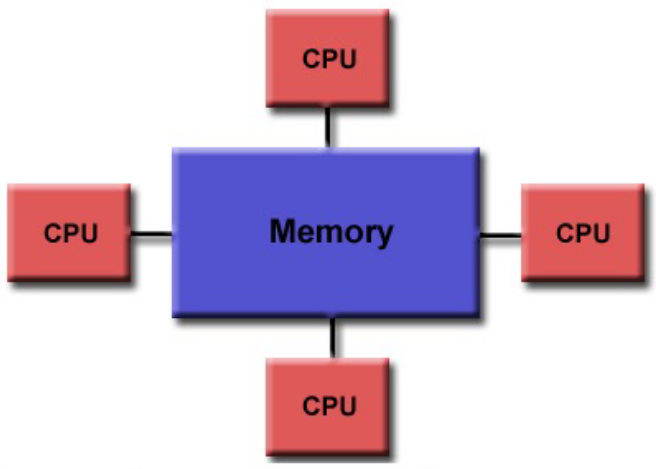
\includegraphics[width=0.7\linewidth]{img/shared-memory}
	\caption{shared memory classe UMA.}
	\label{fig:shared-memory}
\end{figure}
Uniform Memory Access (UMA): oggi più comunemente rappresentato da Macchine Symmetric
Multiprocessor (SMP). I processori sono identici, i tempi di accesso e il modo in cui si accede alla memoria sono gli stessi. A volte chiamato \textbf{CC-UMA (Cache Coherent UMA)}. \textit{Cache coherent} significa che se un processore aggiorna una posizione nella memoria condivisa, tutti gli altri processori sono a conoscenza dell'aggiornamento. La cache coherent è realizzata a livello hardware.
\subsubsection{NUMA}
\begin{figure}[th]
	\centering
	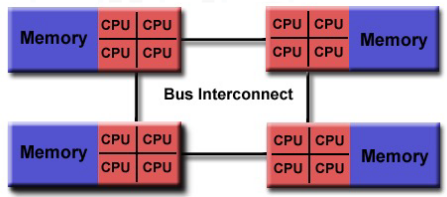
\includegraphics[width=0.7\linewidth]{img/numa}
	\caption{shared memory classe NUMA.}
	\label{fig:numa}
\end{figure}
L'accesso alla memoria non uniforme (NUMA) viene spesso realizzato collegando fisicamente due o più SMP. Un SMP può accedere direttamente alla memoria di un altro SMP. Non tutti i processori hanno lo stesso tempo di accesso a tutte le memorie. L'accesso alla memoria attraverso il collegamento è più lento. Se viene mantenuta la coerenza della cache, può anche essere chiamato \textbf{CC-NUMA --
Cache Coherent NUMA}.
\subsection{Vantaggi e svantaggi delle memorie condivise}
\subsubsection*{Vantaggi}
\begin{itemize}
	\item Lo spazio di indirizzamento globale fornisce una prospettiva di programmazione user-friendly
	per la memoria.
	\item La condivisione dei dati tra le attività è veloce e uniforme grazie alla
	prossimità della memoria alle CPU.
\end{itemize}
\subsubsection*{Svantaggi}
\begin{itemize}
	\item Lo svantaggio principale è la mancanza di scalabilità tra memoria e
	CPU: aggiungere più CPU può aumentare geometricamente il traffico sul percorso memoria-CPU condiviso e, per i sistemi cache coerenti, aumentare geometricamente il traffico associato alla gestione cache/memoria.
	\item  La responsabilità ricade sul programmatore che deve utilizzare i costrutti di sincronizzazione i quali assicurano
	un accesso "corretto" alla memoria globale.
	\item  Diventa sempre più difficile e costoso progettare e
	produrre macchine a memoria condivisa con un numero sempre maggiore di
	processori.
\end{itemize}
\clearpage
\subsection{Memoria distribuita}
\begin{figure}[th]
	\centering
	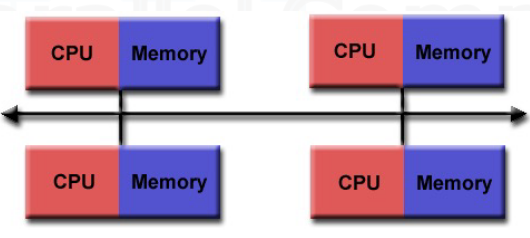
\includegraphics[width=0.7\linewidth]{img/memoria-distribuita}
	\caption{memoria distribuita.}
	\label{fig:memoria-distribuita}
\end{figure}
I sistemi di memoria distribuita richiedono una rete di comunicazione per connettere la memoria interprocessore. I processori hanno la loro memoria locale. Gli indirizzi di memoria in un processore non sono mappati su un altro processore, quindi non esiste un concetto di spazio di indirizzamento globale tra tutti i processori. Poiché ogni processore ha la propria memoria locale, funziona
indipendentemente. Le modifiche apportate alla memoria locale non hanno
effetto sulla memoria di altri processori. Quindi, \textbf{il concetto di
coerenza della cache non si applica}.
Quando un processore ha bisogno di accedere ai dati in un altro processore,
di solito è compito del programmatore definire esplicitamente come
e quando i dati vengono comunicati. Anche la sincronizzazione tra le attività
è responsabilità del programmatore.
La rete utilizzata per il trasferimento dei dati varia ampiamente,
anche se può essere formata da semplici collegamenti Ethernet.

\subsubsection*{Vantaggi}
\begin{itemize}
	\item La memoria è scalabile con il numero di processori. Aumentando il numero di processori, la dimensione della memoria aumenta proporzionalmente. 
	\item Ogni processore può accedere rapidamente alla propria memoria senza
	interferenze e senza il sovraccarico sostenuto nel tentativo di
	mantenere la coerenza della cache.
	\item Efficienza dei costi: può utilizzare processori e reti commerciali e off-the-shelf.
\end{itemize}
\subsubsection*{Svantaggi}
\begin{itemize}
	\item Il programmatore è responsabile di molti dei dettagli associati alla comunicazione dati tra processori.
	\item Potrebbe essere difficile mappare le strutture dati esistenti, basate sulla memoria globale, a questa organizzazione della memoria.
	\item Tempi di accesso alla memoria non uniforme (NUMA).
\end{itemize}
\clearpage
\subsection{Memoria distribuita ibrida}
\begin{figure}[th]
	\centering
	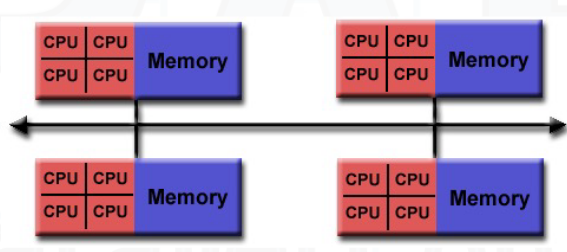
\includegraphics[width=0.7\linewidth]{img/memoria-distribuita-ibrida}
	\caption{memoria distribuita ibrida.}
	\label{fig:memoria-distribuita-ibrida}
\end{figure}
I computer più grandi e veloci del mondo oggi impiegano sia architetture di memoria condivisa che distribuita. Il componente di memoria condivisa è solitamente una macchina SMP coerente con la cache. I processori su un dato SMP possono indirizzare la memoria di quella macchina come globale. Il componente di memoria distribuita è la rete di più SMP.
Gli SMP conoscono solo la propria memoria, non quella di un altro
SMP. Pertanto, sono necessarie comunicazioni di rete per spostare i dati da
un SMP all'altro.
 Le tendenze attuali sembrano indicare che questo tipo di architettura di memoria continuerà a prevalere e ad aumentare nella fascia alta dell'informatica, probabilmente anche in futurp.
\subsubsection*{Vantaggi e svantaggi}Qualunque cosa sia comune sia alle architetture di memoria condivisa che a quelle distribuite.

\section{Modelli di programmazione parallela}
Esistono diversi modelli di programmazione parallela di uso comune.
\subsection{Panoramica}
Sebbene possa non sembrare ovvio, questi modelli non sono
specifici per un particolare tipo di macchina o architettura di memoria. Infatti, uno qualsiasi di questi modelli può (teoricamente)
essere implementato su qualsiasi hardware sottostante. Due esempi:
\begin{enumerate}
	\item  Modello di \textbf{memoria condivisa} su una macchina a \textbf{memoria distribuita}:
	\begin{itemize}
		\item  Approccio ALLCACHE di Kendall Square Research (KSR). La memoria della macchina era distribuita fisicamente, ma appariva all'utente come una
		singola memoria condivisa (spazio di indirizzamento globale). In genere, questo
		approccio è definito "memoria condivisa virtuale".
	\end{itemize}
	\item  Modello di \textbf{passaggio di messaggi} su una macchina a \textbf{memoria condivisa}:
	\begin{itemize}
		\item  MPI su SGI Origin. SGI Origin ha impiegato il tipo  di
		architettura di memoria condivisa CC-NUMA, in cui ogni attività ha accesso diretto alla
		memoria globale. Tuttavia, la capacità di inviare e ricevere messaggi
		con MPI, come avviene comunemente su una rete di macchine a memoria distribuita, non è solo implementata, ma è anche molto
		utilizzata.
	\end{itemize}
\end{enumerate}
\subsection{Modello shared memory}
Nel modello di programmazione a memoria condivisa, le attività condividono uno spazio di indirizzamento comune, che leggono e scrivono in modo asincrono. Vari meccanismi come blocchi/semafori possono essere utilizzati per controllare l'accesso alla memoria condivisa. Un vantaggio di questo modello dal punto di vista del programmatore è che manca la nozione di "proprietà" dei dati. Non c'è bisogno di specificare esplicitamente la comunicazione dei dati tra le attività. Lo sviluppo del programma spesso può essere semplificato. Uno svantaggio importante in termini di prestazioni è che diventa più difficile comprendere e gestire la località dei dati. Mantenere i dati locali al processore che li elabora conserva gli accessi alla memoria, gli aggiornamenti della cache e il traffico del bus che si verifica quando più processori utilizzano gli stessi dati. Sfortunatamente, il controllo della località dei dati è difficile da comprendere e al di fuori del controllo dell'utente medio.
\subsubsection*{Implementazione}
Nelle piattaforme a memoria condivisa, i compilatori nativi
traducono le variabili del programma utente in indirizzi di memoria effettivi, che sono globali.
Attualmente non esistono implementazioni comuni di piattaforme a memoria distribuita. Tuttavia, come menzionato in precedenza nella sezione Panoramica,
l'approccio KSR ALLCACHE ha fornito una vista di memoria condivisa dei dati, anche se la memoria fisica della
macchina era distribuita.
\subsection{Modello delle threads}

Nel modello di programmazione parallela dei thread, un singolo processo può avere più percorsi di esecuzione simultanei. Forse l'analogia più semplice che può essere utilizzata per descrivere le thread è il concetto di un singolo programma che include un certo numero di subroutine:
\begin{figure}[th]
	\centering
	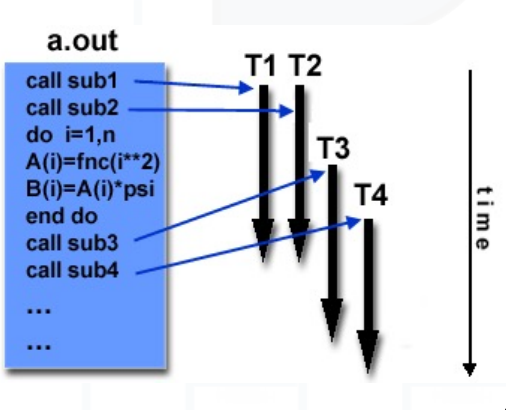
\includegraphics[width=0.4\linewidth]{img/modello-thread}
	\caption{modello delle thread.}
	\label{fig:modello-thread}
\end{figure}

\begin{itemize}
	\item Il programma principale a.out è programmato per essere eseguito dal sistema operativo nativo. a.out carica
	e acquisisce tutte le risorse di sistema e utente necessarie per l'esecuzione.
	\item a.out esegue un lavoro seriale e quindi crea un certo numero di attività
	(thread) che possono essere programmate ed eseguite dal sistema operativo contemporaneamente.
	\item Ogni thread ha dati locali, ma condivide anche tutte le risorse di a.out.
	Ciò consente di risparmiare il sovraccarico associato alla replica delle risorse di un programma
	per ogni thread. Ogni thread trae vantaggio anche da una vista della memoria globale
	perché condivide lo spazio di indirizzamento di a.out.
	\item Il lavoro di una thread può essere descritto al meglio come una subroutine all'interno del programma
	principale. Qualsiasi thread può eseguire qualsiasi subroutine contemporaneamente ad altre thread. 
	\item Le thread comunicano tra loro tramite la memoria globale (aggiornando
	le posizioni degli indirizzi). Ciò richiede costrutti di sincronizzazione per garantire che
	più di una thread non stia aggiornando lo stesso indirizzo globale in qualsiasi
	momento.
	\item Le thread possono andare e venire, ma a.out rimane presente per fornire le risorse necessarie condivise
	fino al completamento dell'applicazione.
\end{itemize}
\subsubsection*{Implementazione}
Le thread sono comunemente associate alle architetture di memoria condivisa e ai sistemi operativi.
Da una prospettiva della programmazione, le implementazioni delle thread comunemente
comprendono:
\begin{itemize}
	\item una libreria di subroutine che vengono chiamate dall'interno del codice sorgente parallelo;
	\item un set di direttive del compilatore incorporate nel codice sorgente seriale o parallelo.
\end{itemize}
In entrambi i casi, il programmatore è responsabile della determinazione di tutto
il parallelismo.
Le implementazioni delle thread non sono una novità nell'informatica.
 Storicamente, i fornitori di hardware hanno implementato le proprie
versioni proprietarie di thread.
 Queste implementazioni differivano sostanzialmente l'una dall'altra, rendendo
difficile per i programmatori sviluppare applicazioni thread portatili.
Sforzi di standardizzazione non correlati hanno portato a due implementazioni di thread molto diverse:
 \begin{enumerate}
 	\item thread POSIX;
 	\item OpenMP.
 \end{enumerate}
 
 \subsubsection{Thread POSIX}
 Basato su libreria;
  richiede codifica parallela.
 Specificato dallo standard IEEE POSIX 1003.1c (1995).
 Solo linguaggio C.
 Comunemente noto come Pthread.
 La maggior parte dei fornitori di hardware ora offre Pthread oltre
 alle loro implementazioni di thread proprietarie.
 Parallelismo molto esplicito;
  richiede una notevole attenzione ai dettagli da parte del programmatore.
  
  \subsubsection{OpenMP}
  Basato su direttiva del compilatore;
   può usare codice seriale.
  Definito congiuntamente e approvato da un gruppo di importanti fornitori di hardware e software per computer.
   L'API Fortran OpenMP è stata rilasciata il 28 ottobre 1997.
   L'API C/C++ è stata rilasciata alla fine del 1998.
  Portabile/multipiattaforma, incluse le piattaforme Unix e Windows NT
  Disponibile nelle implementazioni C/C++ e Fortran
  Può essere molto facile e semplice da usare - fornisce
  "parallelismo incrementale". Microsoft ha la sua implementazione per i thread, che non è correlata allo standard UNIX POSIX o OpenMP.
  
\subsection{Modello di passaggio dei messaggi}
\begin{figure}[th]
	\centering
	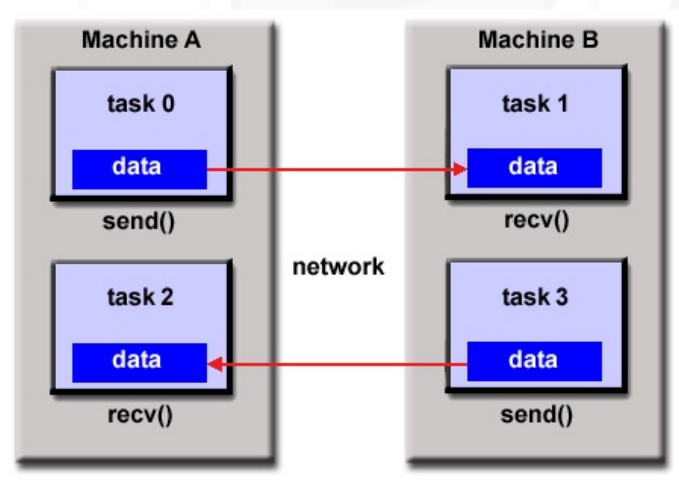
\includegraphics[width=0.7\linewidth]{img/modello-di-passaggio-dei-messaggi}
	\caption{modello di passaggio dei messaggi.}
	\label{fig:modello-di-passaggio-dei-messaggi}
\end{figure}

Il modello di passaggio dei messaggi dimostra le seguenti
caratteristiche:
\begin{itemize}
	
	\item un set di attività che utilizzano la propria
	memoria locale durante il calcolo. Più
	attività possono risiedere sulla stessa
	macchina fisica e anche su un numero arbitrario
	di macchine;
	\item le attività scambiano dati tramite
	comunicazioni inviando e
	ricevendo messaggi;
	\item il trasferimento dei dati richiede solitamente
	che ogni processo esegua
	operazioni cooperative. Ad esempio, un'operazione di invio
	deve avere un'operazione di ricezione
	corrispondente.
\end{itemize}
\subsubsection*{Implementazione}
Da una prospettiva di programmazione, le implementazioni di passaggio di messaggi
comprendono comunemente una libreria di
subroutine che sono incorporate nel codice sorgente.
 Il programmatore è responsabile della determinazione di tutto
il parallelismo.
Storicamente, una varietà di librerie di passaggio di messaggi
sono state disponibili fin dagli anni '80.
 Queste implementazioni differivano sostanzialmente
l'una dall'altra, rendendo difficile per i programmatori sviluppare
applicazioni portabili.
Nel 1992, è stato formato il MPI Forum con l'obiettivo primario di stabilire un'interfaccia standard per le implementazioni di passaggio di messaggi.

MPI è ora lo standard industriale "de facto" per il passaggio di messaggi,
sostituendo praticamente tutte le altre implementazioni di passaggio di messaggi utilizzate
per il lavoro di produzione.
 La maggior parte, se non tutte, delle piattaforme di elaborazione parallela più diffuse offrono almeno
un'implementazione di MPI. Alcune offrono un'implementazione completa di MPI-2.
Per le architetture a memoria condivisa, le implementazioni MPI di solito non
utilizzano una rete per le comunicazioni delle attività. Utilizzano la memoria condivisa
(copie di memoria) per motivi di prestazioni.
\subsection{Modello parallelo dei dati}
\begin{figure}[th]
	\centering
	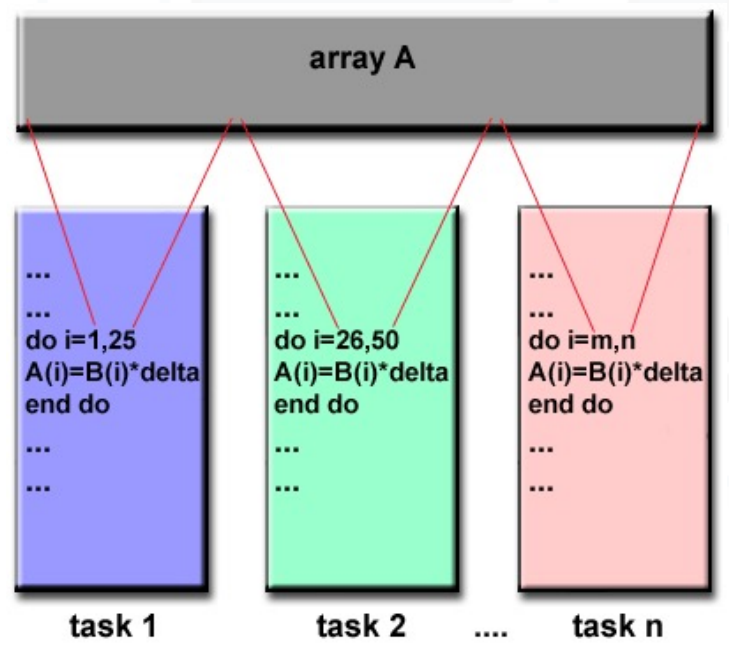
\includegraphics[width=0.7\linewidth]{img/modello-parallelo-dei-dati}
	\caption{modello parallelo dei dati.}
	\label{fig:modello-parallelo-dei-dati}
\end{figure}

Il modello parallelo di dati dimostra le seguenti caratteristiche:
\begin{itemize}
	\item La maggior parte del lavoro parallelo si concentra
	sull'esecuzione di operazioni su un set di dati.
	Il set di dati è in genere organizzato in
	una struttura comune, come un array
	o un cubo.
	\item Un set di attività lavora collettivamente sulla
	stessa struttura di dati, tuttavia, ogni
	attività lavora su una partizione diversa della
	stessa struttura di dati.
	\item Le attività eseguono la stessa operazione sulla
	loro partizione di lavoro, ad esempio,
	"aggiungi 4 a ogni elemento dell'array".
\end{itemize}
Nelle architetture a memoria condivisa, tutti i task possono avere accesso alla
struttura dati tramite memoria globale. Nelle architetture a memoria distribuita, la struttura dati è suddivisa e risiede come "blocchi"
nella memoria locale di ciascun task.
\subsubsection*{Implementazione}
La programmazione con il modello parallelo di dati viene solitamente eseguita scrivendo un programma con costrutti paralleli di dati. I costrutti possono essere chiamate a una libreria di subroutine parallele di dati o direttive del compilatore riconosciute da un compilatore parallelo di dati.
\subsection{Modello ibrido}	È una combinazione dei modelli presentati precedentemente. Ad esempio:
\begin{itemize}
	\item combinazione del modello di passaggio dei messaggi con con il modello delle thread (thread POSIX) o il modello di memoria condivisa (OpenMP);
	\item combinazione del modello dei dati paralleli con il modello di passaggio dei messaggi.
\end{itemize}
\subsection{Modello SPMD -- Single Program Multiple Data}
\begin{figure}[th]
	\centering
	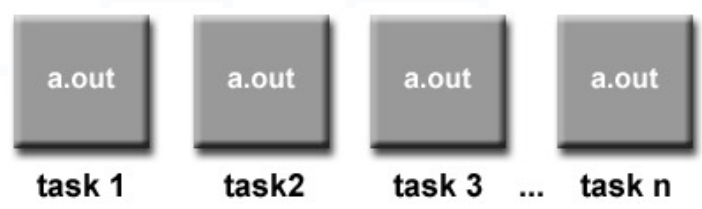
\includegraphics[width=0.7\linewidth]{img/spmd}
	\caption{modello SPMD.}
	\label{fig:spmd}
\end{figure}

SPMD è in realtà un modello di programmazione "di alto livello" che può essere costruito
su qualsiasi combinazione dei modelli di programmazione parallela menzionati in precedenza.
Un singolo programma viene eseguito da tutte le attività simultaneamente.
In qualsiasi momento, le attività possono eseguire le stesse o diverse
istruzioni all'interno dello stesso programma.
\subsubsection*{SPMD vs SIMD}
In SPMD, più processori autonomi eseguono simultaneamente lo stesso
programma in punti indipendenti, anziché nel lockstep che SIMD impone
su dati diversi.
 Con SPMD, le attività possono essere eseguite su CPU per uso generale; SIMD richiede
processori vettoriali per manipolare flussi di dati.
 SPMD è una sottocategoria di MIMD.
I programmi SPMD di solito hanno la logica necessaria programmata al loro interno per
consentire a diverse attività di ramificarsi o eseguire in modo condizionale solo quelle parti del
programma che sono progettate per eseguire. Vale a dire, le attività non devono necessariamente
eseguire l'intero programma, forse solo una parte di esso.
Tutte le attività possono utilizzare dati diversi.
\subsection{Modello MPMD -- Multiple Program Multiple Data} 
\begin{figure}[th]
	\centering
	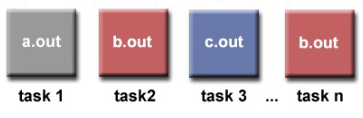
\includegraphics[width=0.7\linewidth]{img/mpmd}
	\caption{modello MPMD.}
	\label{fig:mpmd}
\end{figure}

Come SPMD, MPMD è in realtà un modello di programmazione "di alto livello" che
può essere costruito su qualsiasi combinazione dei modelli di programmazione parallela menzionati in precedenza.
Le applicazioni MPMD in genere hanno più file oggetto eseguibili
(programmi). Mentre l'applicazione viene eseguita in parallelo, ogni attività
può eseguire lo stesso programma o un programma diverso rispetto ad altre attività.
Tutte le attività possono utilizzare dati diversi.